\documentclass[12pt]{examnotes}

\header{DSC3702 International Trade}
%%%%%%%%%%%%%%%%%%%%%%%%%%%%%%%%%%%%%%%
\begin{document}

\obeylines
\h{DSC3702 International Trade}

\h{Study Unit 1}
\sh{Globalisation}
\ra Instant communication, and quick travel (video conferencing)
\ra Tastes are converging. (Coke)
\ra Many imported goods and components, and foreign provided services (Foreign radiographers)
\ra Locals firms facing increased competition from global firms 
\ra Migrant skilled labour, moving local jobs abroad (labour intensive to china)
\ra Globalised financial markets where crises spread quickly (pension funds invested abroad)
\ra Impacts on consumers, workers, investors and voters
\ra Comparable to the industrial revolution, but over a shorter time frame.
\ra Timeline. Spread of Roman coins, Later 19th Century industrial revolution, post world war 2 (reduced trade barriers), 1980's (even more reduced trader barriers and rapid communication, financial flows, travel)
\ra Cons, increase labour movement leads to local jobs losses, increased financial risks, running out of resources and climate change, world poverty, child labour.
\ra Has many social, political, ethical and legal aspects.
\ra Pros: increase efficiency 
 
{\bf Gravity Model} postulates that, ceteris paribus, the bilateral trade between two countries is proportional to the product of the two countries GDP's and smaller the greater the distance between the two countries.

\sh{Explain how a stimulation of the United States economy will affect the South African economy.}

\sh{Describe the main features of international trade in South Africa.}

\sh{Explain the main economic problems and challenges faced by the world economy.}

\sh{Discuss the advantage and disadvantages of globalization.}


\h{Study Unit 2}

\sh{Mercantilism}
\ra Export more than imports, receiving precious metals in return. 
\ra Governments promoted economic nationalism at the expense of other nations.
\ra Measured wealth of nation by stock of precious materials.
\ra More gold meant more money,power,armies and more business activity.
\ra Encouraging exports and restricting imports stimulated national output and employment.
\ra Strict government controls.
\ra Alive and well today in the form of domestic subsidies and trade restrictions.


Gains from trade: The increase in consumption resulting from specialisation in production.
Pattern of trade: The commodities exported and imported by each nation.

\sh{Absolute Advantage}
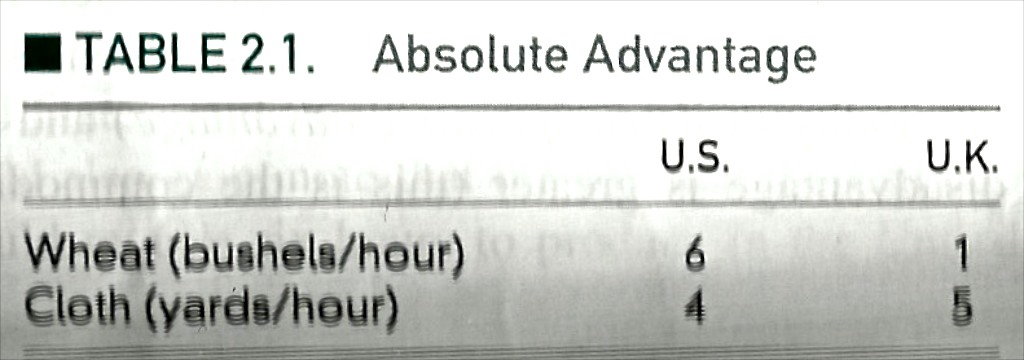
\includegraphics[scale=0.2]{./imgs/t21.jpg}
\ra If nation \emph{1} is more efficient has absolute advantage in commodity \emph{A} and nation \emph{2} has absolute advantage in \mbox{commodity \emph{B}} then both nations gain by specialising and exchanging part of their outputs.
\ra Resources are utilised more efficiency and output of both commodities will rise.
\ra Prompted free trade and laissez-faire governmental policies to increase world welfare and maximise resource utilisation.
\ra Advocated protection of industries necessary for defense.
\ra Contrasted against trade restrictions benefiting few at the expense of many.
\ra Served the interest of factory owners in lower wages (cheaper food imports) but harmed landowners (because food is less scarce) 
\ra A special case of the more general theory of comparative advantage.
\ra Numerical example of exchanging US absolute advantage of 6W for UK 6C with absolute 
\ra Patterns of trade: Export commodities of absolute advantage
\ra Gains from trade: Increased consumption of imported commodities.

\sh{Comparative Advantage}
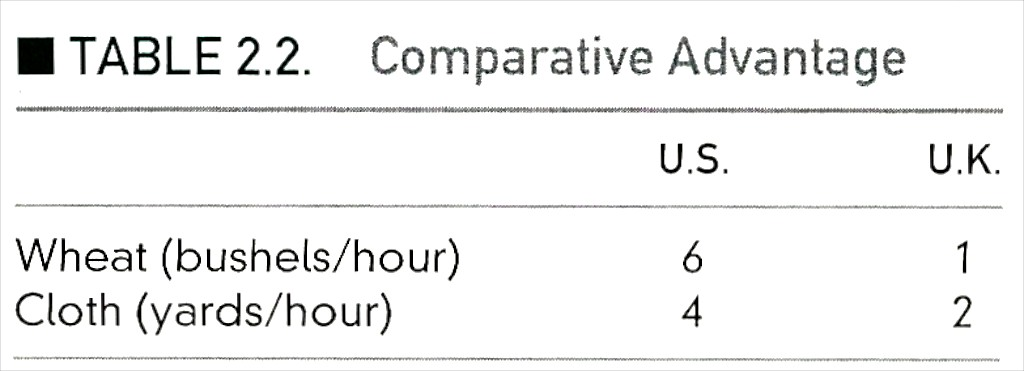
\includegraphics[scale=0.2]{./imgs/t22.jpg}
\ra Assumptions can relax 1-6, but 7 is invalid:
\rn{1} 2 nations and 2 commodities
\rn{2} Free Trade
\rn{3} Perfect mobility of labour in each nation but not between nations
\rn{4} Constant costs of production 
\rn{5} No transportation costs
\rn{6} No technical change
\rn{7} Labour theory of value
\ra Even if one nation has an absolute disadvantage in the production of both commodities there is still a basis for mutually beneficently trade.
\ra Specialise and export in the absolute disadvantage that is smaller, and import the commodity in which the absolute disadvantage is greater.
\ra Two-nation, two-commodity world if one has a comparative advantage the other has a disadvantage.
\ra Both nations can from trade even if one is less efficient than the other in production of both commodities.
\ra Patterns of trade: Export commodities of competitive advantage
\ra Gains from trade: Increased consumption of imported commodities.

\sh{Equal advantage or no comparative advantage}
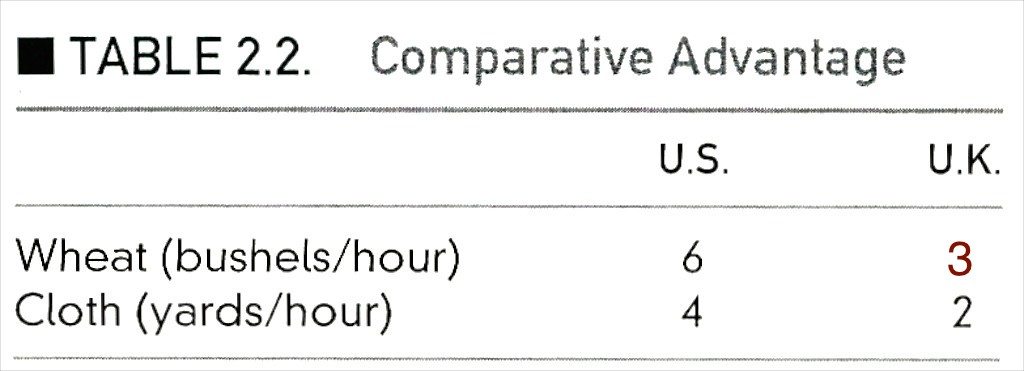
\includegraphics[scale=0.2]{./imgs/t23.jpg}
\ra No comparative advantage if the absolute disadvantage is in the same proportion for both commodities.
\ra Can be created by natural trade barriers such as transport costs even if comparative advantage exists. 
\ra Patterns of trade: Neither country would export commodities
\ra Gains from trade: There would be no increased consumption.

----
\ra Lower productivity generally means lower wages and a reason for trade.
\ra Exchange rates have bearing on the price goods and influence patterns of trade.

\sh{Comparative Advantage and Opportunity Costs}
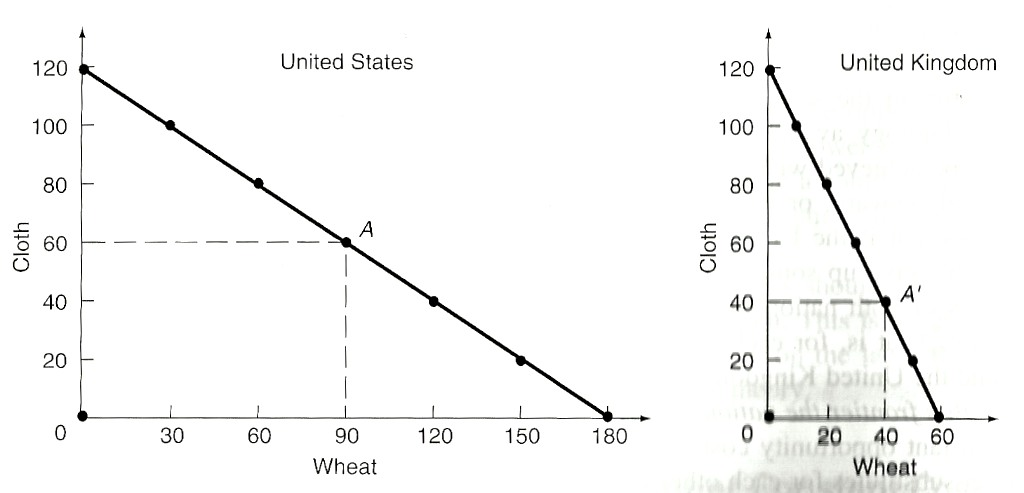
\includegraphics[scale=0.4]{./imgs/21.jpg}
\ra Labour theory of value states that the value or price of a commodity depends exclusively on the amount labour used in production. Which implies:  
\rn{1} labour is the only factor of production or used in same fixed proportions. Labour is clearly not the only factor nor is it used in a fixed proportion. More capital per worker for steel versus textiles. 
\rn{2} labour is homogeneous. Varies greatly in wages, training, productivity.
\ra Opportunity cost theory. The cost of a commodity is the amount of a second commodity that must be given up to release just enough resources to produce an additional unit of the first commodity.
\ra A nation with the lower opportunity cost will have the higher comparative advantage.

----
\ra Constant opportunity costs arise when 
\rn{1} resource or factors of production are either prefect substitutes or used in fixed proportions 
\rn{2} all units of the same factor are homogeneous or of the exact same quality.
\ra $\displaystyle\frac{P_W}{P_C}$ is relative commodity price and is only determine by supply considerations for each nation and demand consideration do not enter at all.
\ra In the absence of trade the production possibly frontier represents the consumption frontier, as the nation can only consume what it produces.

\sh{Basis for gains from trade under constant costs}
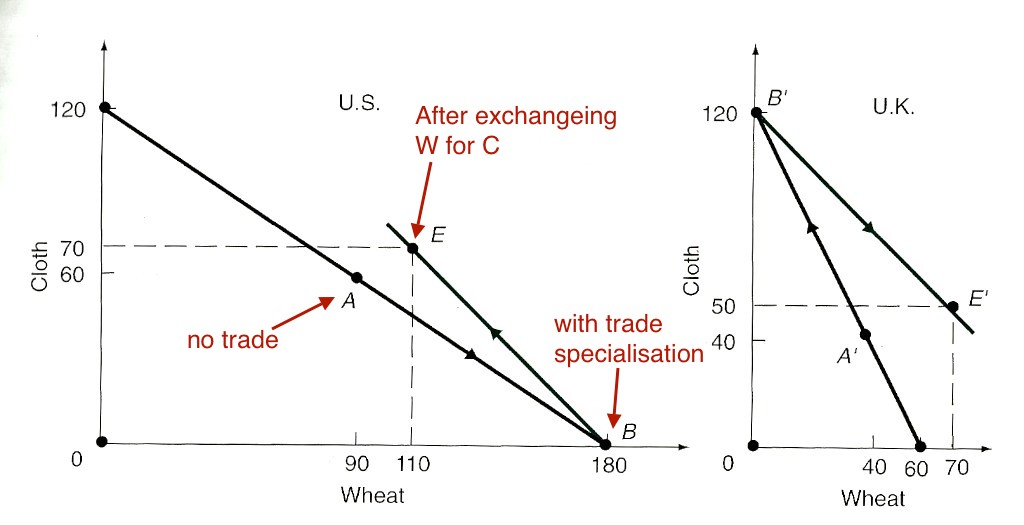
\includegraphics[scale=0.4]{./imgs/22c.jpg}

\sh{Empirical Test of the Ricardian Model}
\ra MacDougall first test using US and UK exports to check relationship between labour productivity and exports. His findings supported the Ricardian theory. The actual pattern of trade is based on the different labour productivities in different industries in the two nations. 

\sh{Criticisms of the classical theory} 
\ra Does not explain the reasons for trade based on differences in productivity. 
\ra Makes extreme predictions that are not fulfilled in the real world. It predicts, for example, that countries will specialise entirely in the production of export goods and ignore the production of import-competing goods. 
\ra Also suggests that the greatest gains from trade occur between dissimilar countries. But the greatest proportion of international trade takes place between industrialised, developed countries which have similar standards of living and similar levels of technology.
\ra Some criticisms are based on the unrealistic assumptions of the classical theory, this criticism does not necessarily invalidate the classical theory. The assumption that there are only two goods can be modified to allow for the more realistic case of trade in more than two commodities where products are ranked by their comparative cost.
\clearpage

\h{Study Unit 3}
Increasing costs of favouring one products over another, or comparative advantage in increasing output.

\sh{Production frontier increasing costs}
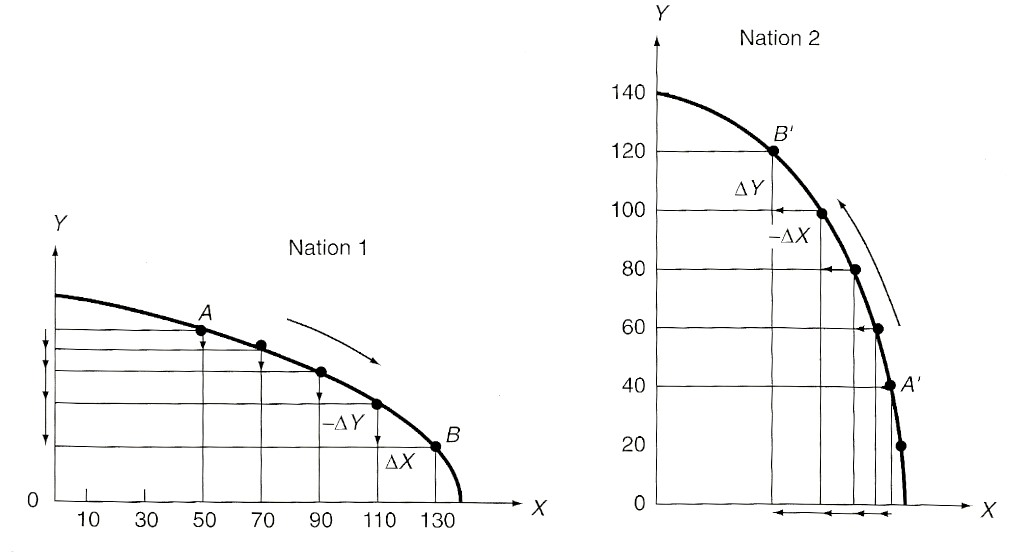
\includegraphics[scale=0.4]{./imgs/31.jpg}
\ra Increasing costs a nation must give up increasing amounts of one commodity to release enough resourced to produce each additional unit of another commodity 
\ra Concave from the origin. 
\ra Slope of PPC is the marginal rate of transformation and is the amount of output that a nation must give up in a specific product, to produce a 1 unit increase in the output of a different product, same as opportunity cost of good.
\ra Increases going up or down because of increasing opportunity costs in production of both products..
\ra The production frontiers nations have different shapes due to the nations having different factor endowments and/or use different technologies. Will usually always differ. Supply and availability cause a shift in the production frontier.
\ra Increasing opportunity costs are due to:
\rn{1} non-homogeneous production factors (quality)
\rn{2} non-constant input weightings, not fixed proportions (quantity)
\ra Some resources are less efficient or less suited to particular products resulting in increasing costs.
\ra Example mountains grazing and flat wheat.

\sh{Community indifference curves}
\ra Various combinations of two commodities that yield equal satisfaction to the nation.
\ra Negatively sloped and convex from the origin.
\ra Marginal rate of substitution is the amount of Y that a nation could give up for one extra unit of X and still remain on the same indifference curve.
\ra Higher indifference curve higher utility.
\ra Compensation principle: The nation benefits from trade if the gainers would be better off even after fully compensation the losers for their losses. 

\sh{Equilibrium in isolation/autarky}
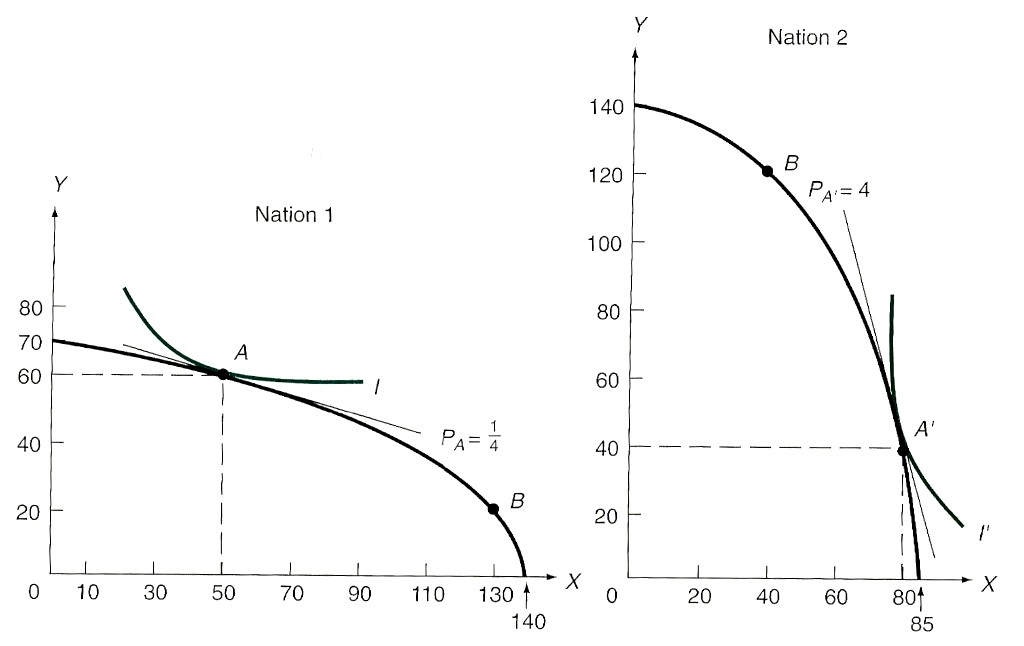
\includegraphics[scale=0.4]{./imgs/34.jpg}
\ra Supply conditions (production possibility frontier) and demand conditions (community indifference curves)
\ra Nation attains equilibrium and maximises welfare at highest possible indifference curve subject to its production possibility frontier at the point of tangency. Can be lower but not maximum cannot be higher due to production constraints.
\ra Slope of tangent is the internal equilibrium-relative commodity price and reflects the nations comparative advantage. $\frac{P_X}{P_Y}$
\ra Nation 1 is in equilibrium at $A$ and Nation 2 at $A \prime$
\ra Relative prices are different in the two nations because their production frontiers and indifference curves different in shape and location.
\ra The forces of supply (PPC) and demand (indifference curves) both determine the equilibrium-relative commodity price.
\ra The Different internal equilibrium commodity prices in that nations indicates that they can engage in mutually beneficent trade.

\sh{Gains from trade with increasing costs.}
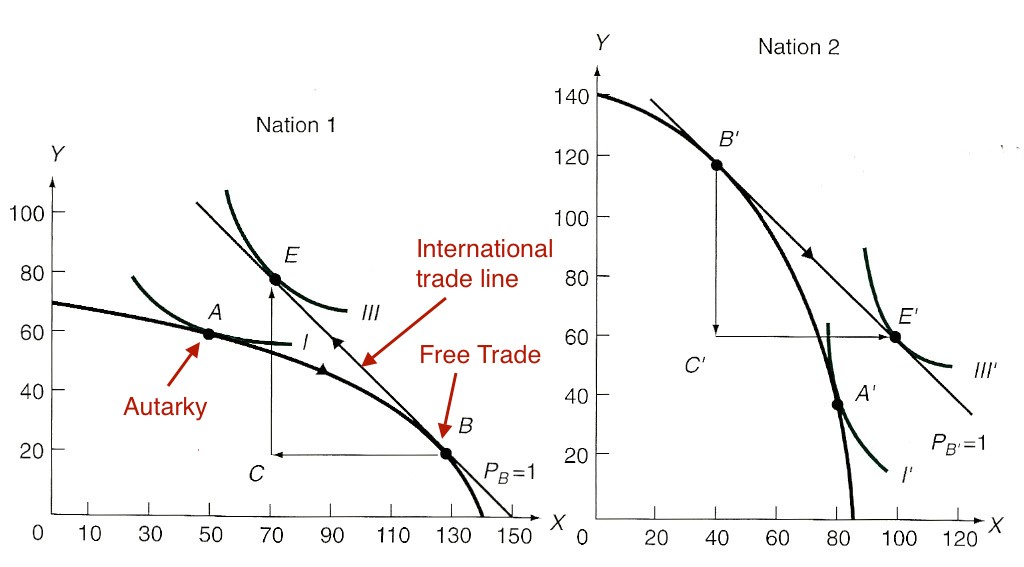
\includegraphics[scale=0.4]{./imgs/35.jpg}
\ra The difference in relative prices indicates comparative advantage and is the basis for mutually beneficial trade between the two nations. 
\ra Each nation will specialize in the commodity of its comparative advantage and export the surplus of that commodity for the other commodity. 
\ra Specialization will continue in the presence of increasing costs until relative commodity prices in the two nations become equal at the level at which trade is in equilibrium. At that point each nation will be consuming more than before trade.
\ra In the absence of trade $P_A<P_{A'}$ with N1 having a comparative advantage X.
\ra With free trade N1 specialises in production of X, exporting and exchange with Y form N2.Nation 1 moves from point A to point B in production.
\ra Each nation will now be consuming on the international terms of trade line.
 Nation 1 will now consume at point E, which is on a higher indifference curve compared to point A. On the other hand nation 2 ends up consuming at point E’. 
\ra The lines PB=PB’=1 represent the equilibrium-relative price at which trade is balanced. N1 exports exactly what N2 demands and vice versa. At any other relative price trade will not be balanced and the relative price will change towards its equilibrium value. 
\ra Under increasing costs there is incomplete specialisation in production in both nations. As each nation specializes in the commodity of its comparative advantage, relative commodity prices move toward each other until they are identical in both nations and this happens before complete specialization.
\ra Each nation consumes outside it PPC.
\ra The equilibrium-relative price with trade is the common relative prices at which trade is balanced.

\sh{The Gains from Exchange and from Specialization}
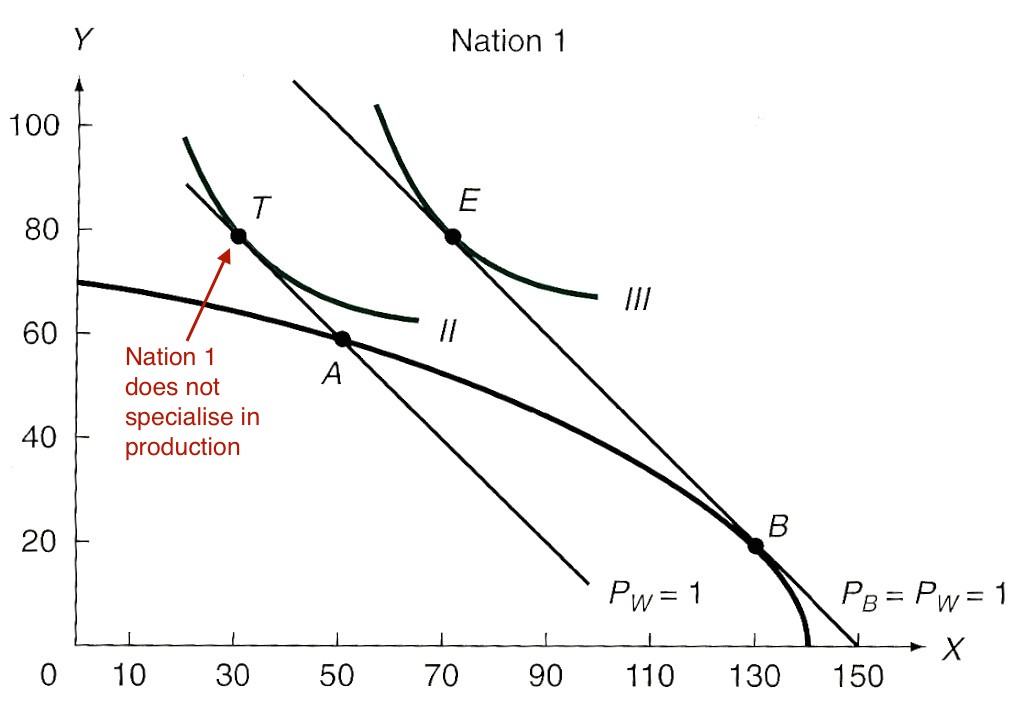
\includegraphics[scale=0.35]{./imgs/25.jpg}
\ra A nations gains from trade are made up of two components: the gains from exchange and the gains from specialization. 
{\bf For a small country}
\ra The movement from point A to point T in consumption measures the gains from exchange.
\ra The movement from point T to point E measures the gains from specialization in production.
\ra Nation 1 is not in equilibrium at point $A$ because $MRT < P_W$, it would need to expand production to point $B$ 

\h{Study Unit 4}

\sh{Heckscher-Ohlin Theory: Assumptions}
\rn{1}Two countries, two homogeneous commodities (X and Y) and two homogeneous factors of production (capital and labour), relatively different initial fixed levels.
\quad\quad\ra Used merely to be able to illustrate model, replacing this assumption leaves conclusion unchanged.
\rn{2} Technology/production techniques is the same in both countries.
\quad\quad\ra If relative factor prices were the same producers in the two countries would use the same quantities of each factor otherwise they use the cheapest factor.
\rn{3} Different factor intensities. Commodity X is labour intensive and commodity Y is capital intensive in both countries. Thus, the two goods are produced with different and uniquely-ordered intensities which are not subject to reversals over all relative factor prices.
\quad\quad\ra Commodity X has a higher $L/K$ ratio than Y in both countries for the same relative prices.
\rn{4} Production incorporates both factors, constant returns in both nations.
\quad\quad\ra Double input double outputs, linear response.
\rn{5} Tastes and preferences are the same in both countries.
\quad\quad\ra shape and location of indifference curves is identical in both nations.
\rn{6} Perfect competition exists in commodity and factor markets.
\quad\quad\ra Perfect information, economics agents to small to affect prices, no economic rent
\rn{7} Factors are perfectly mobile within each country, but not between the countries.
\quad\quad\ra Labour and capital move from low earning areas to higher earning areas in the nation only and International differences in factor earnings would persist indefinitely without trade.
\rn{8} There are no transport costs, tariffs, or other impediments to the free flow of international trade.
\quad\quad\ra Production proceeds till relative and absolute commodity prices are the same in both nation with trade.
\rn{9} All resources are fully employed in both nations.
\rn{10} International trade between the two countries is balanced.
\quad\quad\ra Totals value of import equals total value of exports.
\rn{11} Incomplete specialisation.
\quad \ra Even with free trade both country produce both commodities.  

\sh{Factor intensity.}
\ra Commodity Y is capital intensive if the capital-labour ratio (K/L) used in productions of Y is greater then K/L used in the production of X
\ra Not the absolute amount but only the ratio is important.
\ra If the relative price of capital fall producers will substitute labour for capital in both X and Y but Y will remain the capital intensive product.

\sh{Factor abundance}
\ra Two Definitions
\rn{1} Physical definition (supply side). if the TK/TL ratio is higher in one nation then that nation is capital abundant. Ratio size and not absolute quantities. Only in terms of supply.
\rn{2} Defined in terms of relative factor prices. In terms of the rental price of capital land the price of labour. In terms of demand and supply9.
\ra Read study guide notes.

\sh{Factor abundance and the shape of the production frontier}
\ra Read study guide notes.

\sh{Factor endowments and the factor proportions theory}
\ra Read study guide notes.

\sh{Heckscher-Ohlin theorem}
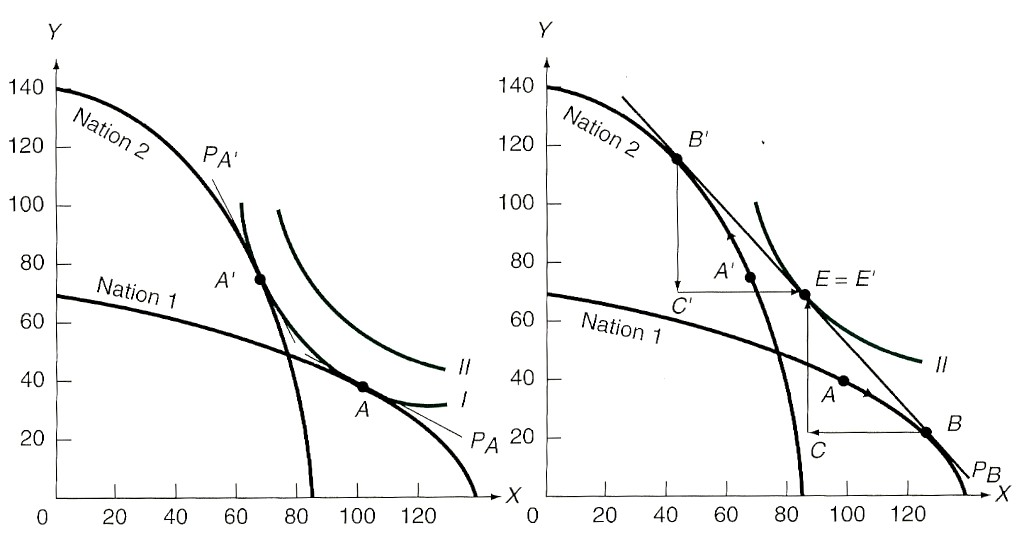
\includegraphics[scale=0.4]{./imgs/54.jpg}
\ra A nation will export the commodity whose production requires the {\bf intensive} use of the nation's relatively {\bf abundant} and cheap factor and import the commodity whose production requires the intensive use of the nation's relatively scarce and expensive factor. 
\ra Factor endowments theory.

\sh{Factor - price equalization and income distribution}
\ra International trade will bring about equalisation in the relative and absolute returns to homogeneous factors of production across nations. As such international trade is a substitute for the international mobility of factors. 
\ra With trade and specialisation, Nation 1 will produce more of commodity X and less of commodity Y. More labour will be demanded and this will raise the wage rate (w) and the relative demand of capital will fall which reduces the interest rate (r). and the opposite will happens in the other nation therefore they move towards the same relative price.
\ra International trade keeps expanding until relative commodity prices are completely equalised, which also means equal relative factor prices in the two nations.

\sh{Effect of trade on the Distribution of Income: The Stolper-Samuelson Theorem}
\ra Since both factors of production are assumed to remain fully employed before and after trade, the real income of labour and the real income of the owners of capital move in the same direction as the movement in factor prices.
\ra This theorem states that the internal distribution of income will change in favour of each country's relatively abundant factor of production.

\sh{The Specific-Factors Model}
\ra Trade will have an ambiguous effect on the nations mobile factors
\ra Trade will benefit the immobile factors specific to the nation's export commodities or sectors
\ra Trade will harm the immobile factors specific to the nation's import-competing commodities or sectors.

\sh{Empirical Relevance}
\ra Many simplifying assumptions don't hold, such as not the same technology, barriers to trade exist, imperfect competition, non-constant returns to scale.
\ra International trade has not equalised homogeneous factors but has only reduced them.
\ra Factor Equalisation theorem does not say differences in per capita incomes will be reduced.

\sh{The Leontief Paradox}
\ra USA was believed to be the most K-abundant nation in the world. Leontief expected the USA to export K-intensive commodities and import L-intensive commodities. 
\ra He estimated K/L ratios for U.S import substitutes and U.S exports using input-output tables for 1947. 
\ra His result stated that U.S import substitutes were more K-intensive than U.S exports, the US  exported more L-intensive commodities and imported more K-intensive commodities. 
\ra His result were opposite to the H-O model predictions
\ra Explanations to the Leontief’s findings.  
(1) the superiority of U.S labour
(2) the human capital
(3) technology explanation (R \& D)
(4) natural resources
(5) factor intensity reversals
(6) inter-country differences in demand or consumption patterns
(7) influence of tariffs.

\sh{Factor Intensity Reversal}
Factor intensity reversal occurs when a given commodity is capital intensive in one nation and L-intensive in the other nation.

\sh{Criticisms of the factor proportions theory}
\ra The theory has little relevance to the real world. 
\ra Leontief paradox 
\ra Demand reversal, when tastes and demand conditions are not identical, they may cause the prices of the same goods to differ substantially from what would be expected on the basis of their relative factor intensities. A disproportionate demand for a nations cheap abundant factor will lead to higher prices and increased imports while exports containing the less abundant factor would increase give the other nations similar disproportionate demand.
\ra Factor intensity reversal, both countries will want to specialise in and export the same commodity. No trade will take place
\ra Demand and factor intensity reversals weaken the conclusions of the factor proportions theory but do not necessarily invalidate it. This would depend on how widespread such contradictions to the theory are in the real world. 
\ra Simplifying assumption of zero transport costs, an unrealistic assumption
\ra Also of concern are the assumptions of perfect competition, constant returns to scale and identical technology. Relaxing these assumptions gives rise to alternative explanations of international trade, which are discussed next.

\sh{International Trade and Economies of scale}
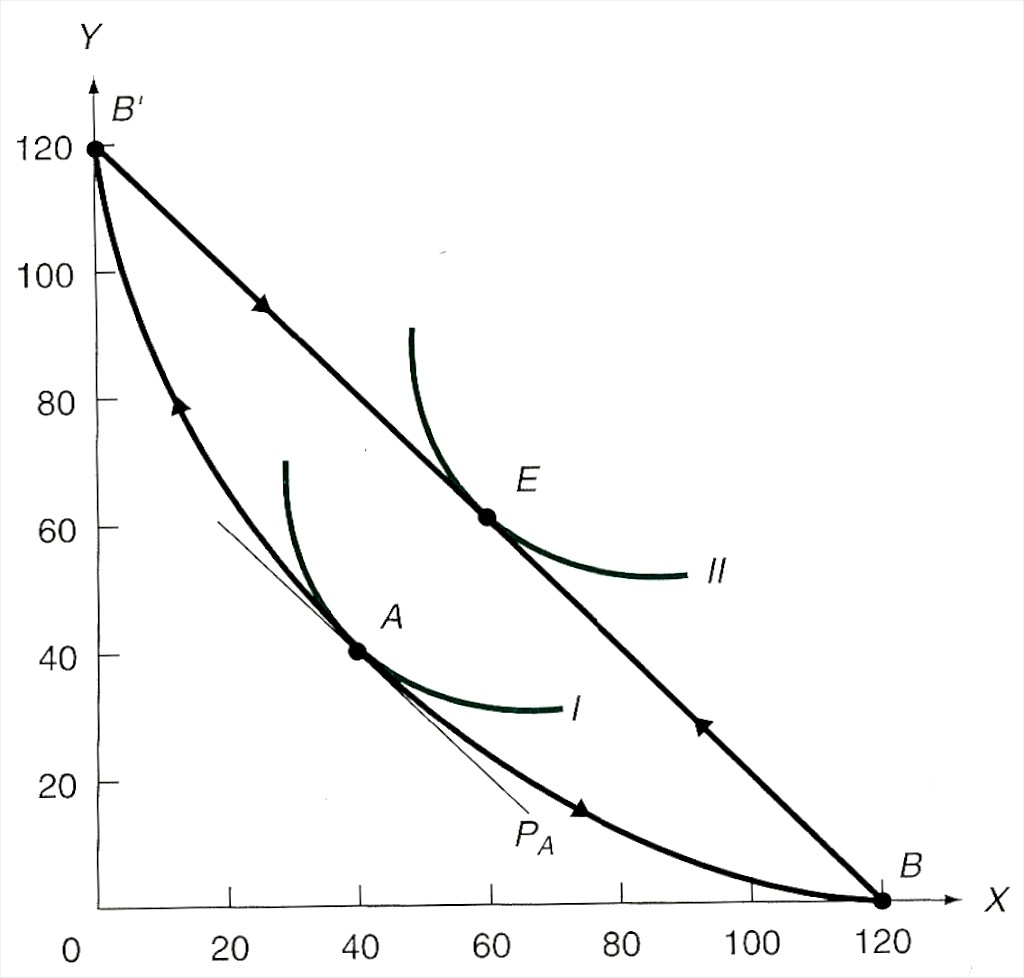
\includegraphics[scale=0.2]{./imgs/61.jpg}
\ra With increasing returns to scale mutually beneficial trade between two countries is still possible. \ra Increasing returns to scale is where output grows proportionately more than the increase in inputs or factors of production. Leads to increased labour productivity due to division of labour and specialization, specialised productive machinery feasible only at a large scale of operation. 
\ra Economies of scale are usually accompanied by extensive product differentiation and theses industries acquire a comparative advantage

\sh{International Trade and Imperfect Competition}
\ra Intra-industry trade occurs when countries both export and import goods from the same industry to and from each other. Germany exports cars to France, but it also imports cars from France. 
\ra The imports and exports are similar. 
\ra It is difficult for the factor proportions theory to explain this because it relies on differences in comparative advantage derived from differences in factor endowments. Germany and France are both developed countries at similar levels of industrialisation, they should have the same advantages and trade between them should be minimal. 
\ra Intra-industry trade arises in order to take advantage of economies of scale in production. It benefits consumers because of the wider range of choices at lower prices made possible by economies of scale in production. 
\ra With differentiated products pre-trade-relative commodity prices no longer accurately predict trade.
\ra With intra-industry trade it is possible for all factors to gain.
\ra Comparative advantage determines inter-industry trade while economies of scale in differentiated products gives rise to intra-industry trade.
\ra The level of intra- industry trade is measured by the intra-industry trade index $T=1-\frac{|X_M|}{X+M}$
\ra The value of the index varies from zero to one. 
\ra The higher the T index the higher the level of intra-industry trade in a particular industry. 
\ra Intra-industry trade is likely to be larger among industrial economies of similar size and factor proportions.

\sh{The Technological Gap Model}
\ra This was developed by Posner. 
\ra It says a lot of international trade is based on the introduction of new products and production processes. 
\ra Technological innovation will give the innovating firm and nation a temporary monopoly based on patents and copy rights. 
\ra The model is based on the hypothesized impact of technological lags and leads in product innovation on the pattern of international trade in manufactured products. 
\ra The technological gap between nations may be a basis of profitable trade between them. 
The models argue that comparative advantage is not static but shifts over time as a result of technical change through sustained innovative activity (through R \& D). 
There is a time lag in the imitation process, both domestically and by foreign competitors. 
This is a supply-based theory and contends that the technologically-abundant countries would possess relative advantages in new products over less technologically developed nations.

\sh{The Product Cycle Model}
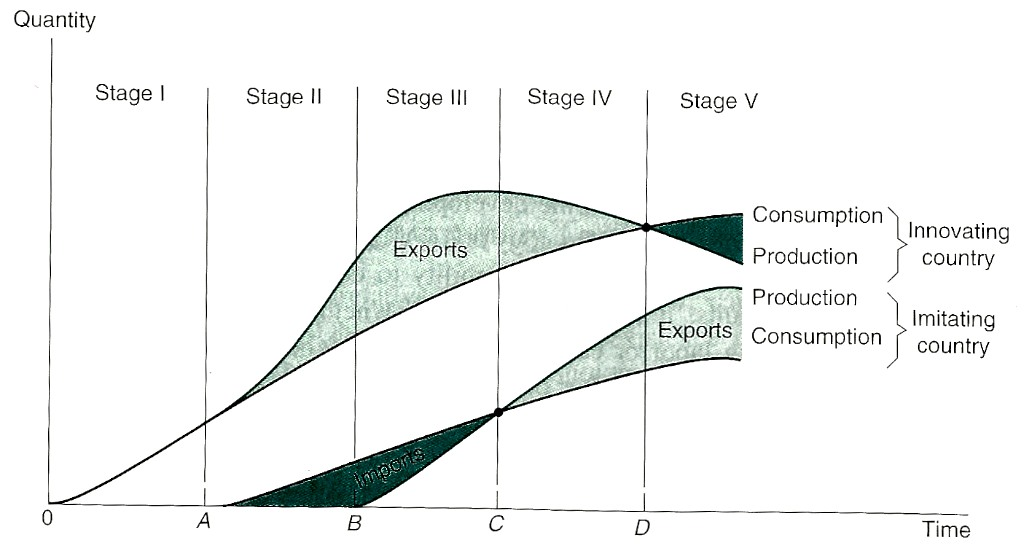
\includegraphics[scale=0.3]{./imgs/64.jpg}
\ra This model is very similar to the technological gap model but stresses product standardization.
\ra Developed by Vernon (1966). 
\ra According to this model when a new product is introduced, it usually requires highly skilled labour to produce. As the product matures and acquires mass acceptance, it becomes standardized; it can be produced by mass production techniques and less skilled labour. 
\ra Over time comparative advantage in the product shifts from the advanced nation that originally introduced it to less advanced nations, where labour is relatively cheap. The innovating country ends up as a net importer of the product they initially introduced on the market.
Do these alternative new trade theories completely discredit the traditional factor proportions theory? In the textbook, the author makes the point that the two approaches explain different aspects of international trade and are thus not mutually exclusive. The factor proportions theory explains inter-industry trade between developed and developing countries reasonably well, whereas the new trade theories are better equipped to explain intra-industry trade between countries at the same level of industrialisation. Also, the basic principle of comparative advantage is still at work in the new trade theories, but they can explain dynamic changes in comparative advantage better than the essentially static analysis of the factor proportions theory. It is argued that the new trade theories are dynamic extensions of the basic H-O model.

\h{Study Unit 5}

\sh{Tariffs}
\ra Levied for protection of domestic industries from foreign competitive, or to raise revenue on export or imports.
\rn{1} Specific tariff, fixed tax or duty per unit
\rn{2} Ad valorem, percentage tax
\rn{3} Compound, combination of specific and ad valorem.

\sh{Partial equilibrium analysis}
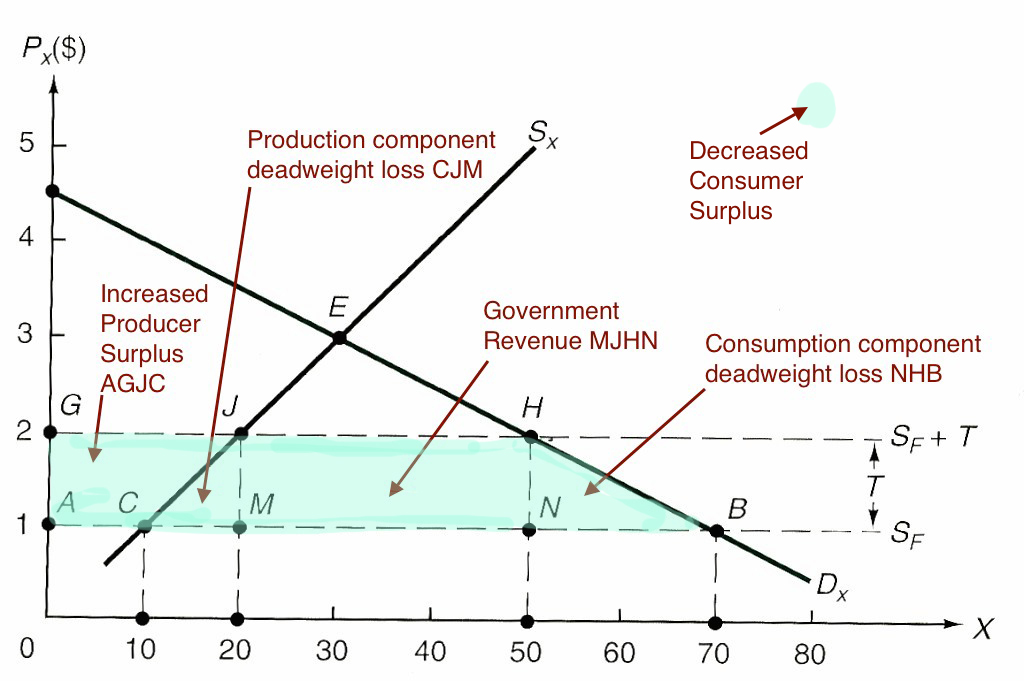
\includegraphics[scale=0.4]{./imgs/81.jpg}
\ra Small country, tariffs does not affect world prices nor the rest of the economy (small industry)
\ra Autarky equilibrium at point E
\ra Free trade at $P_X=1$, with infinitely elastic supply curve $S_F$ nation consumes AB, with AC domestic and CB imported production. 
\ra 100\%  tariff increase price to $P_X=2$, with consumption GH, of which GJ is domestic and GH imported. $S_F + T$ new tariff inclusive foreign supply curve.
\ra Effects.
\rn{1} Consumption effect, reduced domestic consumption BN
\rn{2} Production effect, expansion of domestic production CM
\rn{3} Trade effect, decline in imports  BN+CM
\rn{4} Revenue effect, increase government revenue, MJHN
\ra The more elastic (flatter) demand the greater the consumption affect
\ra The more elastic the supply the greater the production effect.
\ra The more elastic $S_X$ and $D_X$ the greater is the trade affect and the smaller is the revenue affect.

\sh{Effect of tariff on consumer and producer surplus}
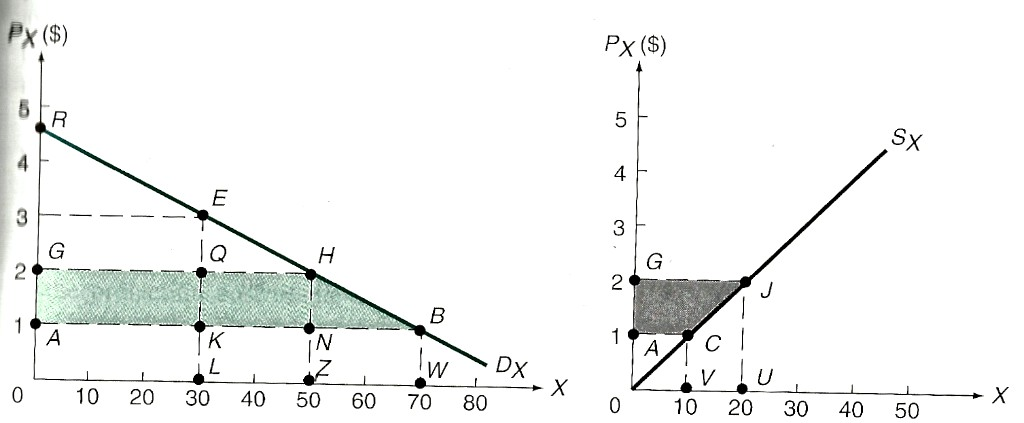
\includegraphics[scale=0.4]{./imgs/82.jpg}
\ra A tariff leads to a reduction in consumer surplus AGHB i.e. from ARB to GRH.
\ra Consumer surplus is the difference between what consumers would be willing to pay for each unit of a commodity and what they do pay.
\ra A tariff leads to an increase in producer surplus ACGH. The subsidy effect of the tariff.

\sh{Cost and Benefits of a tariff}
\ra Use partial equilibrium analysis figure
\ra Decrease consumer surplus
\ra Increased Producer surplus
\ra Protection or deadweight loss, (tariff leading to inefficiencies)
\rn{1} production component. domestic resource are transfer from production of more efficient Y to production of less efficient X.
 \rn{2} consumption competent. because of artificial increase in $P_X$'s distortion on consumption patterns
\ra Increased government revenue
\ra Income is redistributed from domestic consumers to domestic producers of the commodity and from the nation's abundant factor (producing the exportable) to the nation's scarce factor (producing the importable)
\ra dividing loss in consumer surplus by jobs saved gives cost per domestic job.

\sh{Optimum tariff and welfare}
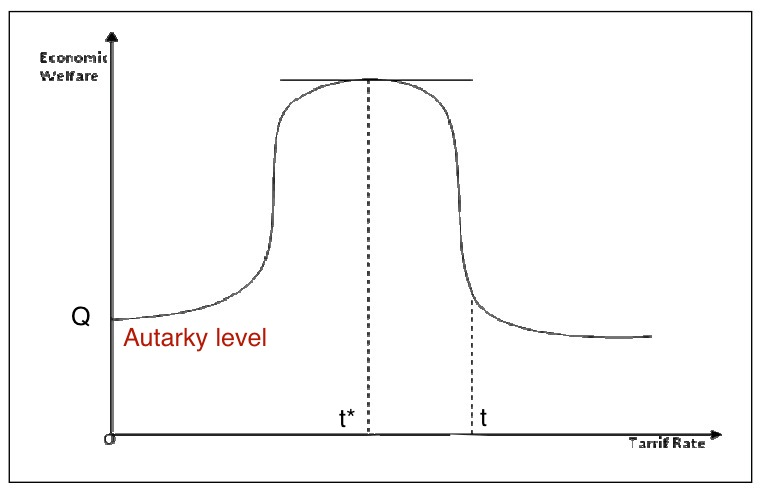
\includegraphics[scale=0.4]{./imgs/532.jpg}
\ra In a large county imposing a tariff has two effects.
\rn{1} Volume of trade decreases reducing the nations welfare
\rn{2} Increase in terms of trade improves nations welfare.
\ra The optimum tariff is the rate of tariff that maximises the net benefit resulting from the important in terms of trade and the reduction on the volume of trade.
\ra Small country optimum tariff is always zero because there is no improvement in terms of trade.
\ra $Q$ is free trade welfare level, with trade and tariff welfare increases to optimum $t^*$ then decrease back to autarky level at $t$ and when tariff is prohibitive country is worse off.
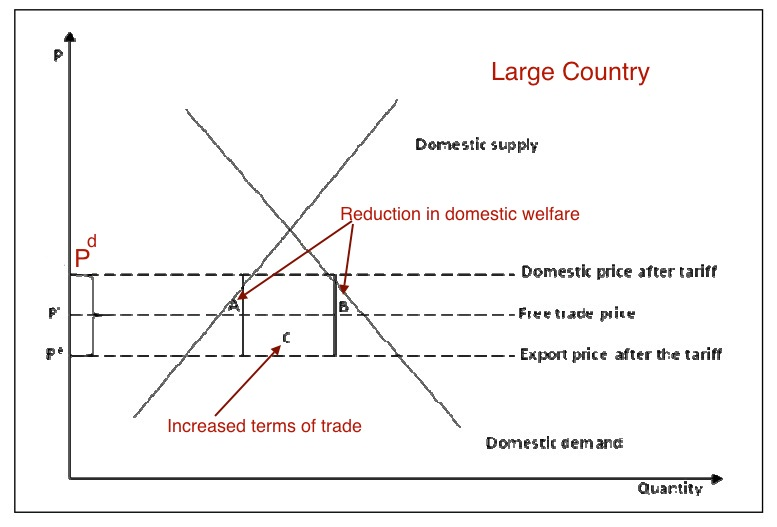
\includegraphics[scale=0.35]{./imgs/531.jpg}
\ra tariff $t$ increase domestic price to $P^d$, because a large country foreign suppliers pay part of tariff $C$ which is an increase in terms of trade. $A$ and $B$ is reduction in domestic welfare. $C -(A+B)$ maximised for net gain is the optimum tariff. 
\ra Other nation are likely to respond with their own tariffs thereby all nations will lose.

\sh{Rate of effective protection}
\ra Effective protective rate for a final product increases 1) as the nominal rate on it increases or 2) the nominal rate on imported inputs decreases
\ra The effective tariff rate of protection is the percentage increase in domestic value added per unit of output made possible by the tariff structure.
\ra The greater the proportion of imported inputs, the greater the difference between nominal rate and the effective rate. 
\ra Applying both a tariff on import inputs and final goods is self-defeating 
\ra Domestic value added equals the price of the final commodity minus the cost of import inputs.
\ra Effective rate  important to producers as indicates how much actual protection is afforded.
\ra $g=\displaystyle\frac{t-a_it_i}{1-a_i}$ $a_i=$ ratio of imported input costs to to final price. $t=$ nominal rate on final goods. $t_i=$ nominal rate on imported inputs 
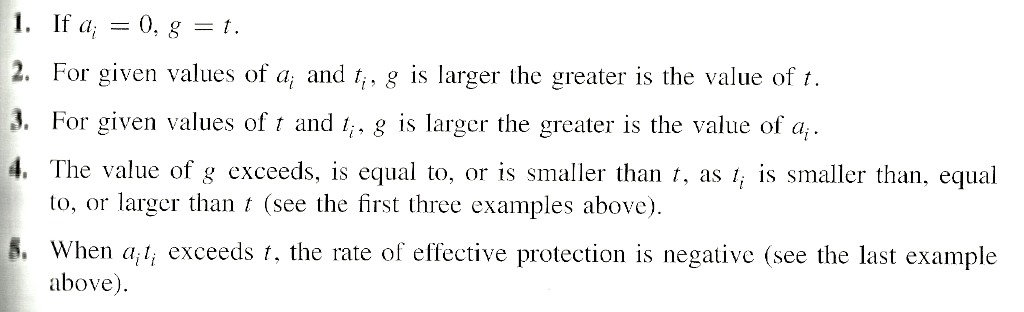
\includegraphics[scale=0.5]{./imgs/53.jpg}
\ra A tariff on imported inputs is a tax on domestic producers increasing costs, reducing effective protection of nominal inputs and discourages domestic production.
\ra Nominal rate is descriptive.
\ra Higher rates tend to be found in labour-intensive industries
\ra Some substitution by produces of tariff increase inputs by cheaper domestic or imported inputs.


\vspace{6pt}
\vspace{6pt}
{\bf \Large Nontarriff trade barriers}
\ra More harmful than tariffs, with export subsidies more harmful than import quotas.
\ra Most prevalent in agriculture.

\sh{Import quotas}
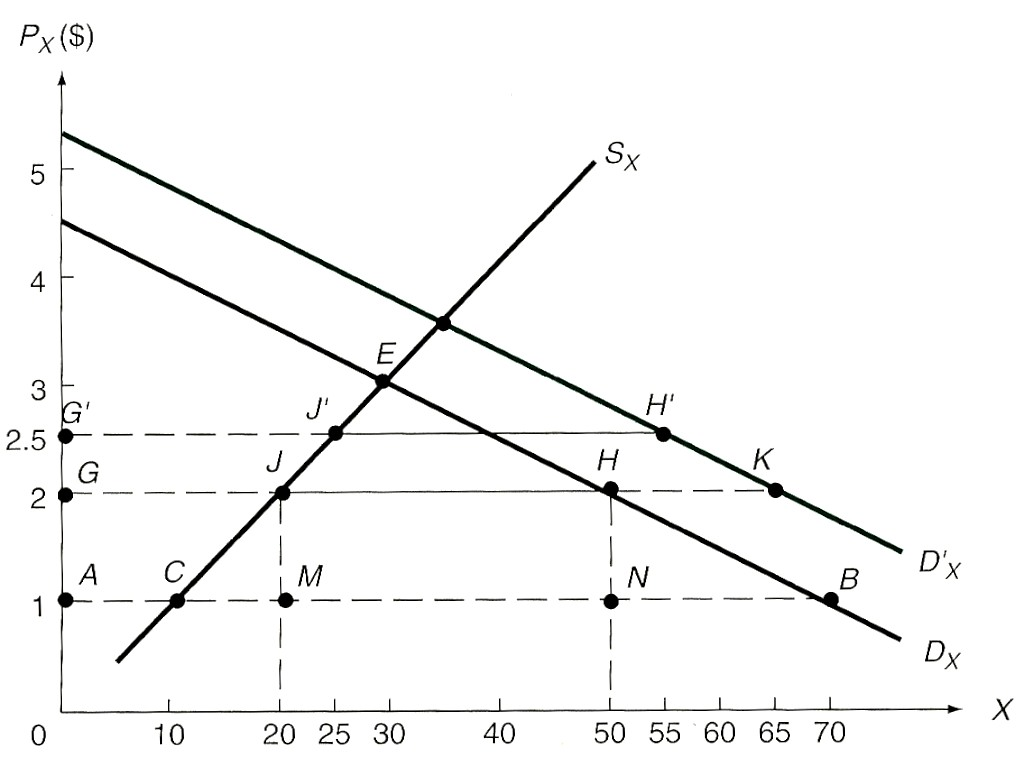
\includegraphics[scale=0.3]{./imgs/91.jpg}
\ra WTO prohibits quotas on manufactured goods.
\ra A direct quantitative restriction on the amount of a commodity allowed to imported or exported.
\ra Used to protect domestic industry. Industrial nations use it to protect agriculture and developing nations use it to simulate import substitution of manufacture goods and balance-of-payments reasons.
\ra Free trade at price $P_X=1$, consuming $AB$ of which $AC$ is local and $CB$ imported.
\ra An import quota of $JH$ increase price to $P_X=2$ same as ad valorem tariff. At this price the import quota plus domestic production equals demand. Domestic production increase to $GJ$ and import decreases to $JH$, same as ad valorem tariff.
\ra Revenue from competitively auctioned import licenses would be $JHMN$
\ra If $D_X$ shifts upward to $D_X^\prime$ the the import quota would increase the domestic price to $P_X=2.5$.

{\bf Comparison of Import Quota and Import tariff}
\ra With a given import quota, an increase in domestic demand will result in a higher domestic price and greater domestic production. i.e affects domestic prices for shifts in supply or demand
\ra With a given import tariff an increase in demand will leave the domestic price and domestic production unchanged but will result in higher consumption and imports. i.e. affect quantity of imports for shift in supply or demand.
\ra Import quota complete replaces market mechanism rather than altering it like a import tariff.
\ra Import quota involves distribution of licenses which results in:
\rn{1} Monopoly profits for firms obtaining licences in uncompetitive manner, including inefficiency due to bureaucratic decision making. a waste for the economy.
\rn{2} Contain the seeds of corruption through rent seeking by importers to obtain monopoly profits.
\rn{3} Limits imports to the specified level with certainty, while trade effect of an import tariff may be less visibly uncertain (exporters could absorb all tariff costs or take lower profits), therefore producers favour import quotas. 
\ra Import quotas are more restrictive and society should resit producer's efforts.

\sh{Voluntary export restraints}
\ra Bilateral agreements between two governments in which the exporting country agrees to limit its exports to the importing country. 
\ra The importing country refrains from imposing more restrictive measures while the VER is adhered to.
\ra  Were quite significant (10\% of world trade), May no longer be used (Since 1999) under the Uruguay Round
\ra Economic effects of an equivalent import quota. 
\ra Administered by the exporting country, therefore revenue effect or rents are captured by foreign exporters. 
\ra Less effective than import quotas, because of reluctance of exporting countries to curb exports, and exporters fill quotas with higher-quality, higher priced units, and transshipments via countries not party to the VER.

\sh{International cartels}
\ra Agreements between foreign companies or governments to restrict output and exports of a commodity with the aim of maximizing or increasing the total profits of the group. 
\ra example OPEC. 
\ra Cartels raise prices by restricting output and exports of the commodity concerned.
\ra The producer countries gain at the expense of the consumer countries. 
\ra Cartels are unstable and difficult to maintain in the long run because of the incentive for individuals to cheat and to raise exports above the agreed limits. 
\ra Free riders (non-participatory countries) benefit from the higher prices and increase output and prices are decreased. 
\ra Likely to only be successful if there are only a few international suppliers of essential commodities and no close substitutes, and then cartels can act like a monopolist.

\sh{Anti-dumping import duties}
\ra Taxes on goods that are deemed to have been imported at prices lower than those for the same good in the exporting country's domestic market. 
\ra Three categories
\rn{1} sporadic: To unload a temporary or unseen surplus without having to reduce domestic prices.
\rn{2} predatory: to drive foreign producers out of business after which prices are raised by new acquired monopoly power
\rn{3} persistent dumping: international price discrimination: Because local market is less accessible to foreign producers can charge higher domestic prices. 
\ra Difficult to decide whether or not dumping has occurred or the type of dumping and domestic producers want protection from any form of dumping.
\ra Implicated countries tend to raise prices rather than face anti dumping duties. 
\ra Anti-dumping import duties are permitted by the WTO, but the importing country has to prove that dumping and injury occurred. 
\ra South Africa has both imposed such duties and had anti-dumping duties imposed on its exports.

\sh{Export subsidies}
\ra Direct payments made by government to a nation's exporters or potential exporters and or low interest loans to foreign buyers to stimulate the nation's exports. 
\ra Not a restriction on trade but gives domestic companies an unfair advantage, helping them to increase their exports at the expense of foreign competitors in world markets. 
\ra A form of dumping and prohibited by the WTO but still provided by nations.
\ra In SA exporters benefited from the General Export Incentive Scheme during the 1980-1990s. South Africa has ended such subsidies as part the Uruguay Round of 1994.
\ra Farmers in developed countries continue to be subsidised. The aircraft industries in the US and the EU are subsidised. Industrial countries also provided low cost loan to finance exports, measured by amount of interest that should have been paid.
\ra Countervailing duties are often imposed on imports to offset export subsidies by foreign governments.
{\bf Partial equilibrium of export subsidy.}
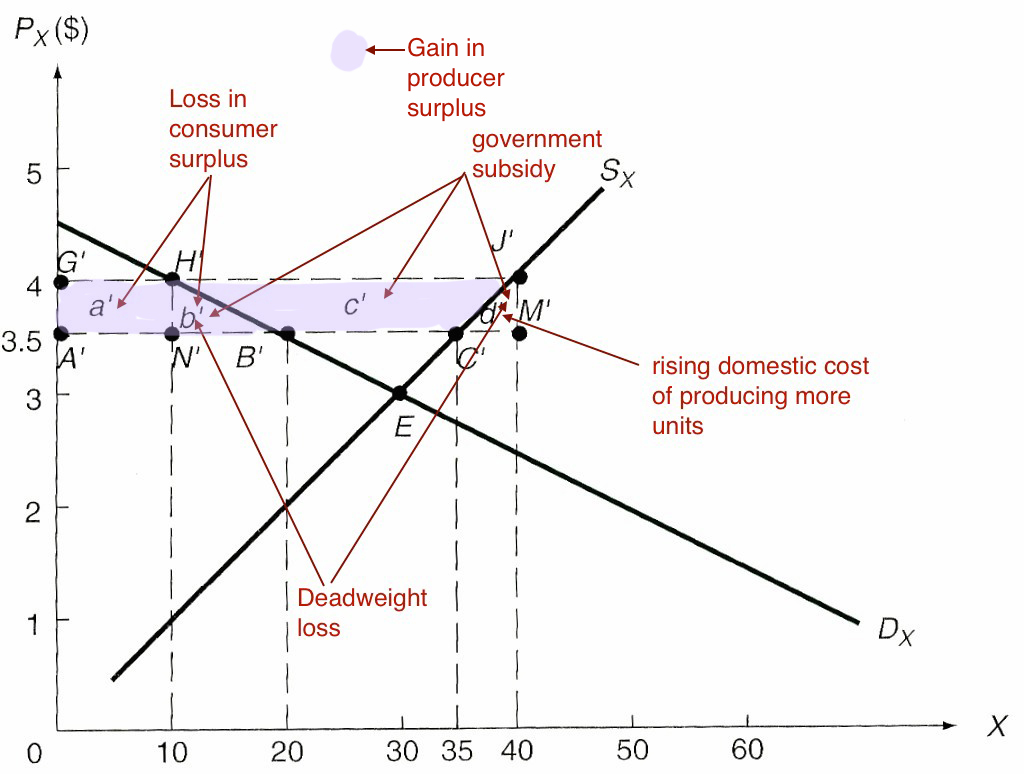
\includegraphics[scale=0.3]{./imgs/92.jpg}
\ra At free trade price $P_X=A\prime$ production is $A\prime C\prime$, consumption is $A \prime B \prime$ and exports are $B \prime C \prime$. Nation is an exporter of commodity $X$.
\ra If the government of the small county provided a subsidy of $0.50$ per unit, $P_X$ rises to $G \prime$ for domestic producers and consumers. Domestic production increase to $G \prime J \prime$ domestic consumption is $G \prime H \prime$ and export are $H \prime J \prime$
\ra *Describe change in consumers surplus, producer surplus and dead weight loss.
\ra The higher price benefits domestic producers but harms domestic consumers. Home nation also incurs the cost of the subsidy. Domestic producers gain less than the sum of the loss to domestic consumers and the cost of the subsidy to the home nation.
\ra Export subsidy occurs due to lobbying from, domestic producers, or the government wishing to promote certain industries.
\ra Foreign consumers gain because they receive a larger quantity at the free trade price.
\ra If the home nation is large it will face a decline in its terms of trade due to the need to reduce $P_X$

\sh{Fallacious arguments for protection}
\rn{1} Trade restrictions are needed to protect domestic labour against cheap foreign labour. Even if domestic wages are higher, domestic labour cost can be lowered through increase labour productivity. Even without increase productivity mutually beneficial trade can take place because of comparative advantage.
\rn{2} The scientific tariff. A tariff rate that would make the price of imports equal to domestic prices allowing domestic producers to meet foreign competition. This however would eliminate international prices differences and trade in all commodities subject to such scientific tariffs.

\sh{Questionable arguments for protection}
\rn{1} Reduce domestic unemployment.  
\rn{2} Correct balance of payment deficits.
\ra Protection, it is argued, would lead to a substitution of imports for domestic production.
\ra Beggar-thy-neighbour arguments as they come at the expensive of other nations, i.e. having the opposite effect on other countries. 
\ra Domestic unemployment and deficits should be corrected with appropriate monetary, fiscal and trade policy.

\sh{Infant-industry and other qualified arguments for protection}
\ra A nation might have a potential comparative advantage in a commodity but lack know-how and small level of output the industry will not be set up or cannot compete successfully with established foreign competition.
\ra Temporary trade retrospection advocated to protect the industry in its infancy until it can achieve economies of scale, meet foreign competition and reflect the nations long run comparative advantage.
\ra The return of the grown-up industry should be successfully high to offset the higher prices paid by domestic consumers.
\ra Qualifications:
\rn{1} Justified more for developing nations than industrial nations as they have undeveloped capital markets.
\rn{2} Difficult to identify qualifying industries and remove the protection at a later stage.
\rn{3} An equivalent production subsidy can be better Production subsides are easier to remove. 
\ra Direct subsides are better than tariffs at, as the infant industry is a domestic distortion and should be dealt with by domestic policy. Subsidies however revenue and don't generate them like an import tariffs does.
\ra Trade restrictions are also advocated for protection of national defence industries, but again direct subsides are better.
\ra Some tariffs are regarded as bargaining tariffs to induce other nations to agree to a mutual reduction in tariffs. 
\ra The optimum tariff argument for large nations.

\sh{Who gets protected}
\ra Stronger incentive for a few producers to lobby for protection than the diffused losses of many consumers.
\ra Protection more likely to be provided to labour intensive industries, employ low-skilled low-wage workers.
\ra Pressure-groups and special interest groups such as highly organised industries.
\ra More protection for industries producing consumer goods than intermediate goods, as consumer production is able to increase prices.
\ra Goes to more geographically decentralised industries that employ a large number of workers.
\ra Protection to maintain the status quo, avoid changes in the distribution of income.
\ra In industrial nations more protection from developing nations exports.

\sh{Strategic trade policy}
\ra Activist trade policy and protectionism. A nation can create a comparative advantage through temporary trade protection,, subsidies, tax benefits and cooperative government-industry programs, in industries such as semi-conductors computers, telecommunication  other other industries deemed crucial for growth.
\ra These industries are subject to high risk, require large scale production to achieve economies of scale and give rise to external economies when successful.
\ra Similar to infant industry argument.
\ra Extremely difficult to pick winners, devise policy for successfully nurture. 
\ra If all leading nations undertake strategic policy they neutralise each other.
\ra Comes at the expense of other nations.

\sh{Compare and contrast the effects of tariffs and quotas.}

\sh{Explain the effect of a tariff on a country's terms of trade.}

\h{Study Unit 6}

\sh{Describe and explain the main principles on which the WTO is based}
\ra Established 1995 and replaces GATT (General Agreement on Tariffs and Trade) with a broader mandate and has 156 Members/
\ra Set and regulates international trade conduct to promote international trade and reduce tariff barriers, including agricultural products.
\ra Members negotiate tariff concessions at conferences called rounds, last one Uruguay round (1986-1993).
\ra Disputes settled by 2/3 or 3/4 majority and not unanimous as in GATT.
\ra Monitors national trade polices
\ra Provides assistance and training for developing countries.
\ra Deals with in transactions in commercial services, intellectual property rights, foreign investment
\ra fundamental principles:
1: Most favoured nation principle. non-discrimination between members,i.e. tariff rates and concessions agreed too  by some members must be extended to all members. Customs Unions and free trade areas are exempt.
2: General prohibition of export subsidies (except for agriculture), general prohibition of import quotas.
3: New tariffs must be offset by reduction in other tariffs.
4: Equal and fair national treatment. Non-discrimination between foreign firms and domestic firms. 
5: Reciprocity, out country will treat your firms the same way your country treats our firms.
6: Mutual recognition. In EU product standards are uniform across members
7: Fast tract voting (trade promotion). In USA voting on negotiated trade agreement without amendments. Expired.
8: Not concerned with environmental issues as it is concerned with products, not process and externalities of production.
\ra Developing country differences: 
1: They receive preferential treatment in industrial countries
2: Reciprocity does not apply.
3: Exempt from prohibition on quotas and export subsidies.

\sh{The Uruguay Round}
\ra Completed in December 1993
\ra Sticky Points:
\rn{1} Disagreements between Us, EU on reducing agricultural subsidies.
\ra Aim was to establish rules for checking the proliferation of new protectionism and reverse the trend, brings services, agriculture and foreign investment into the negotiations, protection of international property rights, improve the dispute settlement mechanism. 
\ra Major provisions:
\rn{1} Tariffs. Tariffs on industrial product were to be reduced, the share of goods on zero tariffs was to be increased, tariffs on pharmaceutical. construction equipment., medical equipment, paper products and steel were removed completely.
\rn{2} Quotas: Quotas on textiles, apparel and agricultural products to be replaced with less restrictive tariffs.
\rn{3} Antidumping: Tougher and quicker action to solve disputes from anti-dumping laws but did not ban their ruse.
\rn{4} Subsidies: Volume of agricultural export  and government industrial research subsidies to be reduced.
\rn{5} Safeguards: Nations could temporary  raise tariffs or other restriction against i,port surge that harmed domestic industry but barred countries from administering health and safety standards without scientific evidence.
\rn{6} Intellectual property: 20 year protection for patents, trademarks and copyrights.
\rn{7} Services: US failed to access Japan, Korea and developing nations for its banks and security firms, or reduce EU restrictions on US films and TV shows.
\rn{8} Other industry provisions: Limiting aircraft subsidies , opening up telephone markets, limiting EU steel maker subsidies, opening of Japanese computer chip market.
\rn{9} Trade-related investment measures: Phase out requirements that foreign investors buy supplies locally or export as much as they import.
\rn{10} WTO: Replacement of General Agreement on Tariffs and Trade GATT with World Trade Organisation, with authority in trader, agricultural products and services.

\sh{Outstanding trade problems and Doha Round}
\ra Continued widespread trade protectionism. Advanced nations protection of domestic jobs. India banned Chinese toys. US, EU subsiding car makers.
\ra Subsidies and tariffs on agricultural products remains very high, Antidumping measures and safeguards are frequently abused.
\ra Tendency of the world to break up into three major trading blocks. EU, NAFTA and less defined Asian bloc leas to bilateral deals, protectionism and inter trade bloc conflicts.
\ra Call by developed countries for the establishment of labour and environmental standards to level working conditions and avoid social dumping. 
{\bf Doha round}
\ra Further liberalisation of production and trade in agriculture, industrial products and services
\ra Further tightening of rules for anti dumping measures and safeguards, investment and completion policies.
\ra Developing nation were reluctant to make concession as they felt that the Uruguay round failed to deliver a great deal of what was promised to them an insist on making the Doha Round a developmental round. 
\ra Doha round collapsed in 2006 and all attempt to revive it failed in 2012 mainly over disagreement about agricultural subsidies.

\sh{Regional Economic Integration}
\ra Economic integration is the commercial policy of discriminatively reducing or eliminating trade barriers only among the nations joining together, such an arrangement discriminates between member and non-member countries. 
\rn{1} Preferential trade agreements reduce tariffs or other trade barriers between the member countries concerned. Each country retains its own trade barriers with non-member countries. eg. British Commonwealth Preference Scheme.
\rn{2} Free trade areas are similar to PTAs, but trade barriers between the member countries are removed completely. As with a PTA, each member country retains its own tariffs and other trade barriers with non-member countries. eg North American Free Trade Agreement (NAFTA), Southern African Development Community (SADC).
\rn{3} Customs unions are FTAs which harmonise their trade policies with the rest of the world, for example by having a common tariff on trade with non-member countries. European Union (EU) began as a customs union with fewer members. The South African Customs Union (SACU) which includes South Africa, Swaziland, Lesotho, Botswana and Namibia. South Africa sets the common external tariff and administers the customs revenue pool. A feature of the SACU is that such revenues are shared unequally between the member countries. The smaller economies get a disproportionately larger share of the pooled revenues. This is to compensate them for the external tariff being decided by South Africa and for the polarisation of industrialisation towards South Africa.
\rn{4} A common market is a customs union which allows factors of production (labour and capital) to move freely between the member countries. Economic Community of Europe in 1993.
\rn{5} An economic union is the most advanced form of economic integration. Besides free trade and mobility of the factors of production, the member countries unify monetary and fiscal policies. eg . Current EU and USA.

\sh{Trade-creating customs Union}
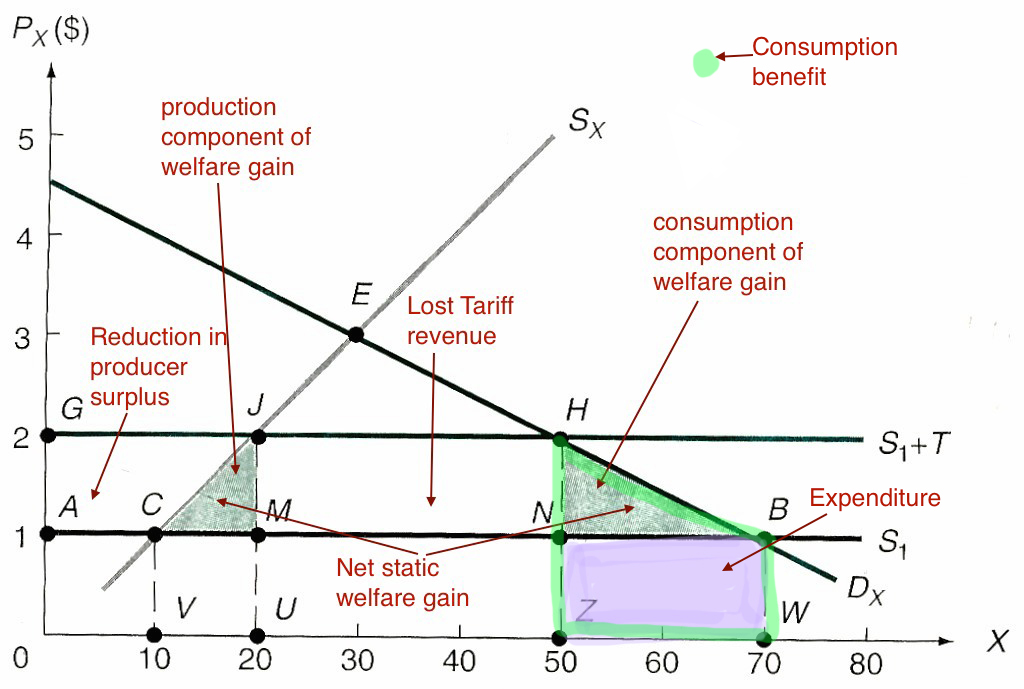
\includegraphics[scale=0.4]{./imgs/101.jpg}
\ra Trade creation occurs when some domestic production in a nation that is a member of a customs union is replaced by lower-cost import from another member nation.
\ra If resources fully employed, increases welfare of member nations due to greater specialisation in production based on comparative advantage.
\ra A trade-creating custom union also increase the welfare of non-members as increases in real income spills over to increased import from rest of world.
\ra Nation 2 i8s too small to affect prices.
\ra Free trade price in Nation 1 is $P_x=1.00$ and rest of world $P_X=1.5$.
\ra If home nation imposes a non-discriminatory 100\% ad valorem tariff then the home nation will import from Nation 1 at $P_X=2$, consuming $GH$ of which $GJ$ is domestic production and $JH$
is imported from nation 1. Nation 2 collects revenue $MJHN$.
\ra Home nation does not import from rest of world because $P_X=3$
\ra If home nation forms a customs union with nation 1 and removes the tariff on import from nation 1 only, then $P_X=1$ and home nations consumes $AB$, of which $AC$ is domestic production and $CB$ is is imported from nation 1.
\ra Consumer surplus increase by $AGHB$, but only partly represents a net gain because $AGJC$ is a reduction producers surplus,  and $MJHN$ is lost revenue. $CJM$ and $HNB$ is the net static welfare gain.
\ra $CJM$ is the production component of welfare gain resulting from shifting production $CM$ from less efficient domestic producers in home nation to more efficient nation 1 producers.
\ra $BHN$ is the consumption component of welfare gain and results from increase in consumption of $NB$ giving a benefit of $ZWBH$ with and expenditure of only $ZWBN$

\sh{Trade-Diverting Customs Union}
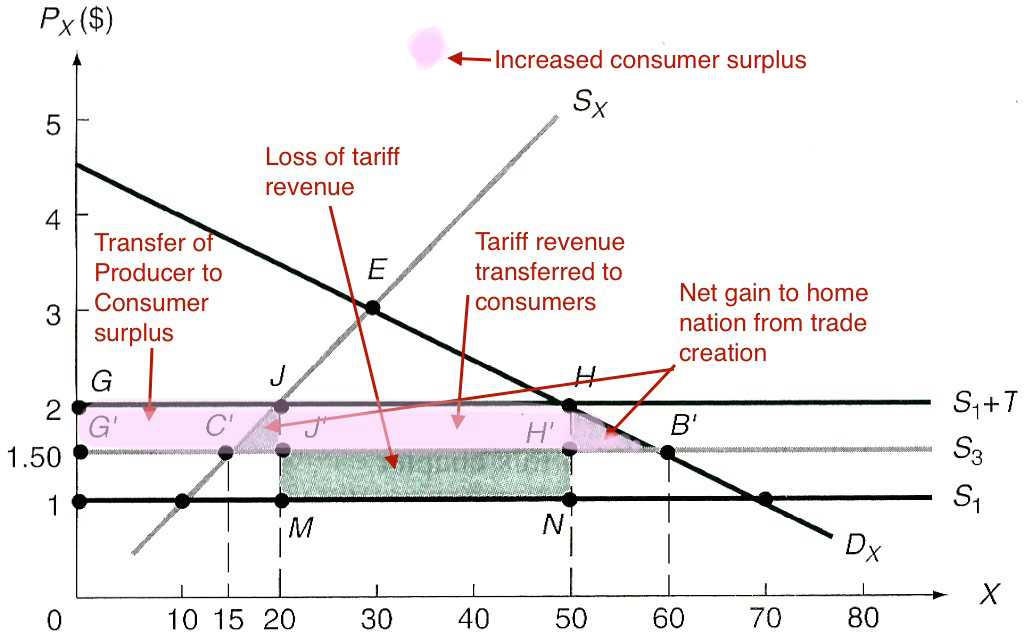
\includegraphics[scale=0.4]{./imgs/102.jpg}
\ra Occurs when lower-cost imports from outside the customs union are replaced by higher cost imported from a union member. 
\ra Reduces welfare because it shifts production from more efficient producers outside the customs unions to less efficient producers inside the customs union.
\ra Worsens international allocation of resources and shifts production away from comparative advantage.
\ra A trader-diverting custom union result in both trade creation and trade diversion and can therefore increase or decrease member welfare.
\ra Demand and supply of home nation $D_X$, $S_X$ with free trade perfectly elastic supply curves $S_1$, $S_3$.
\ra With a nondiscriminatory 100\% tariff on imports of X, $P_X=2$, consumption is $GH$, domestic production is $GJ$ and imports are $JH$ , tariff revenue $JMHN$. 
\ra If home nation forms a customs union with Nation 3 only. Home nations now imports only from N3 at $P_X=1.5$ consumes $G \prime B \prime$ with $G \prime C \prime$ domestic production and $C \prime B \prime$ imported. Home nation collects no tariff revenue and imports have been diverted from more efficient N1 to less efficient N3 because of discriminatory tariff against non-members. Trade creation also occurs from increased import 
\ra Shaded areas are static welfare effects. $C \prime J J \prime$ $B \prime HH$ are trade creation welfare increase, while $MNH \prime J \prime$ is welfare loss from trade diversion of initial $JH$ imports from N1 to N3. $G \prime GHB$ gain in consumer surplus from creation of customs union. $J \prime JHH \prime$ tariff revenue transferred to consumes of home nation.
\ra The lost tariff revenue is larger than the net gain and therefore a net welfare loss to home nation. The more elastic supply and demand would leave a smaller lost tariff revenue and a possible net welfare gain for home nation.

\sh{Theory of second best}
\ra If all conditions required to maximise welfare or reach Pareto optimum cannot be satisfied, trying to satisfy as many of these conditions as possible does not necessary lead the second-best position.
\ra Thus forming a customs union and removing trade barriers only among the members will not necessarily produce the second best welfare position (welfare can rise or fall).

\sh{Conditions more likely to lead to increased welfare for a customs union}
\rn{1} The higher the preunion trade barriers of members the greater the trade creation of a custom union.
\rn{2} The lower are the customs union's trade barriers with non-members, less likely to lead to costly trade diversion. 
\rn{3} The greater the number of members, the greater the probability of low-cost producing members.
\rn{4} The more competitive rather than complementary are the economies of members, the more  opportunities there are for specialisation and trade creation hence greater welfare. 
\rn{5} The closer geographically the members  are will result in lower transport cost are as a barrier to trade.
\rn{6} The greater the preunion trade and economic relationships of potential members. Leads to greater opportunities for signification welfare gains as a result of the formation.
\vspace{-3pt}
\sh{Other static welfare affects of customs unions}
\ra Administrative savings from elimination of customs officers, border patrols. Occurs whether trade creating or trade diverting.
\ra A trade diverting customs union by reducing demands for imports and supply of exports to non-members leads to an improvement in the collective terms of trade.
\ra For trade-creating custom unions leads to a reduction in terms of trade as increased real income spills over to rest of the worlds imports
\ra Customs unions acting as s single unit in international trade nations have more bargaining power, eg. EU.
\vspace{-3pt}
\sh{Dynamic Benefits from customs unions}
\ra Increased competition. Removal of trade barriers amongst members increases competition amongst producers who must either become more efficient, merge or go out of business. Sluggish monopolies and oligopolistic who were complacent behind trader barriers will have to become more efficient, however antitrust legislation would need to be enforced to prevent similar union-wide monopolistic.
\ra Economies of scale. Due to larger market customs union can reduce range of differentiated products and increase product runs. Small nations can however create economies of scale through world trade and do not need to be members of custom union top do so.
\ra Stimulation of investment. Increased investment from enlarge market and increased competition0. Also spurs non-members to open production facilities within union to avoid being left out of market.
\ra In a custom union that is also a common market, great factor mobility will result in better utilisation of factors of production.
\ra Presumed to much greater the static gains. However still second-best solution as unilateral elimination of trade barriers is better but needs to be balanced against reduction in terms of trade.
\ra Strong opposition t0 removal of all barriers by vocal and influential minorities that would be hurt in process.
\ra Some argue regional blocks allow more rapid trade liberalisation, other argue it retards economic liberalisation and lead to inter-bloc conflicts. 
\ra Trading block should strive to reduce external and internal trade barriers and easily admit new members.

\end{document}
